\documentclass[a4paper,spanish,12pt]{article}
\usepackage[spanish]{babel}
\usepackage[utf8]{inputenc}
\usepackage[pdftex]{graphicx}
\usepackage{vmargin}
%\usepackage{algorithmic}
%\usepackage{float}
\usepackage{lastpage}
\usepackage{caratula}
\usepackage{algorithm}
\usepackage{algorithmic}
\usepackage{url}


%%%%%%%%%%%%%%%%%%%%%%%%%%%%%%%%%%%%%%%%%
% ECO Para jugar con el footer. 		%
\usepackage{fancyhdr}					%
%%%%%%%%%%%%%%%%%%%%%%%%%%%%%%%%%%%%%%%%%


%%\usepackage{hyphenat}
%%\exhyphenpenalty=10000
%%\hyphenpenalty=10000
\setmarginsrb{10mm}% left margin
{15mm}% top margin
{15mm}% right margin
{10mm}% bottom margin
{0mm}{20mm}{0mm}{30mm}% we needed -- related to headers and footers

%%%%%%%%%%
\pagestyle{fancy}
\fancyhf{}

\fancyhead[RO, CE]{Teor\'{i}a de las Comunicaciones}
%\fancyhead[LO, CE]{Grupo X}
\fancyfoot[C]{ Página \thepage\ de \pageref{LastPage} }

\renewcommand{\headrulewidth}{0.6pt}
\renewcommand{\footrulewidth}{0.6pt}

\newcommand{\ite}[3]{\textbf{if} #1 \textbf{then} \\ \hspace*{7mm}\vbox{#2} \\ \textbf{else} \\ \hspace*{7mm}\vbox{#3} \\ \textbf{fi} }
\newcommand{\itf}[3]{\textbf{if} #1 \textbf{then} \\ \hspace*{7mm}\vbox{#2} \\ \textbf{fi} \\ }
\newcommand{\whi}[2]{\textbf{while (} #1 \textbf{)} \\ \hspace*{7mm}\vbox{\noindent #2} }
\newcommand{\tades}[2]{\noindent\textbf{TAD} #1 \textbf{ES} #2 \\}
\newcommand{\punt}[1]{($\ast$#1)}
\newcommand{\fle}{$\rightarrow$}


%%%%%%%%%%

\begin{document}


%*************************************************************%
%                                                             %
% CARATULA                                                    %
%                                                             %
%*************************************************************%
    \materia{Teor\'{i}a de las Comunicaciones}

    \titulo{Trabajo Práctico 1b}
  
    %\subtitulo{Tres problemas de programación}

    %\grupo{Grupo 255}

    \integrante{Antonio, Pablo}{290/08}{pabloa@gmail.com}
	\integrante{Ferrari, Gastón}{775/07}{gastonferrari5@hotmail.com}
    \maketitle
    
    \lhead{Trabajo Práctico 2}
    
%*************************************************************%
%                                                             %
% INFORME                                                     %
%                                                             %
%*************************************************************%

	\tableofcontents
	\newpage

\section{Introducción}
\indent En este trabajo practico nos dedicaremos a explorar el nivel de red. Para hacerlo, implementaremos la herramienta Traceroute, para luego usarla para explorar y conocer mas la red.\\
\indent También analizaremos lo compleja que es la red y las caracteristicas de la misma.

\subsection{Traceroute}
\indent Traceroute es una herramienta de diagnóstico que permite seguir la pista
de los paquetes que vienen desde un host (punto de red). Es decir, se envía un
paquete a una dirección IP y por cada router por el que pasa el paquete hasta
llegar al destino, se devuelve un paquete con la información de ese enlace. Asi,
es posible lograr saber por donde pasa un paquete hasta que llega a su destino
final. Se obtiene además una estadística del RTT o latencia de red de esos
paquetes, lo que viene a ser una estimación de la distancia a la que están los
extremos de la comunicación.

\subsection{ICMP}
\indent ICMP (Internet Control Message Protocol) es el sub protocolo de control
y notificación de errores del Protocolo de Internet (IP). Como tal, se usa para
enviar mensajes de error, indicando por ejemplo que un servicio determinado no
está disponible o que un router o host no puede ser localizado. Es importante
destacar que este protocolo no intecambia datos. Los paquetes ICMP viajan dentro
de los paquetes IP como si fueran de un protocolo de nivel superior. 



\newpage

\newpage

\section{Primera Parte: Estimación de RTT}
En esta primera parte del trabajo, el objetivo es realizar mediciones de
\emph{round-trip time} tanto teóricas como empíricas y razonar alrededor de
los resultados.

\subsection{Caracterización de los experimentos}

Elegimos tres universidades en distintas partes del mundo (Cambridge
University, Inglaterra; Stanford University, Estados Unidos; Moscow State
University, Rusia) y, tomando la dirección IP del dominio principal de cada
una, realizamos las siguientes mediciones:
\begin{enumerate}
    \item \textbf{Cálculo del RTT teórico.} Para esto, primero definimos la
        ubicación geográfica de la dirección haciendo uso de un servicio de
        geolocalización. Con ella, calculamos la distancia lineal desde ese
        punto hasta el que sería el origen de nuestras mediciones. Tomando un
        tiempo de propagación de la señal de $2 \times 10^5$ km/s, calculamos
        el tiempo que tardaría la ida de un paquete hasta el servidor destino
        y la llegada de una respuesta o reconocimiento inmediato.
    \item \textbf{Medición de RTT teórico teniendo en cuenta el camino
        recorrido por los paquetes.} Similar al cálculo teórico anterior, esta
        vez teniendo en cuenta las ubicaciones geográficas de cada uno de los
        routers intermedios.
    \item \textbf{Medición de RTT mediante una herramienta propia.} Utilizando
        una herramienta de \emph{traceroute} desarrollada por nosotros usando
        la biblioteca Scapy, calculamos el RTT empírico a la dirección
        destino.
    \item \textbf{Medición de RTT mediante una herramienta del sistema
        operativo.} Idéntico al caso anterior pero esta vez usando el
        \emph{traceroute} disponible en una distribución de GNU/Linux.
\end{enumerate}

Previamente a las mediciones, se esperaba que el RTT teórico lineal fuera, en
general, muy menor a los obtenidos empíricamente, puesto que este, además de
dejar de lado retardos ocasionados por los routers en distintas horas del día,
asumía la existencia de un medio de comunicación (fibra óptica) cubriendo la
menor distancia entre el origen y el destino de la medición. Dado que el RTT
teórico del camino no asume esto último, se esperaba que este, si bien fuera
menor a los valores empíricos, se ajustara más a estos.

Por otro lado, se esperaba ver que los valores de RTT empíricos arrojados por
ambas herramientas de \emph{traceroute} fueran cercanos, ya que las mediciones
se realizarían en condiciones similares y los métodos para realizar los
cálculos serían parecidos.

Asimismo, como realizaríamos mediciones para distintos momentos del día, se
esperaba ver diferencias en los RTT según el horario, aunque no se suponía
ningún patrón en particular.

\subsection{Resultados de los experimentos}

Las figuras \ref{fig:cambridge:count}, \ref{fig:stanford:count} y
\ref{fig:msu:count} muestran las mediciones para la Cambridge University
(Inglaterra), Stanford University (Estados Unidos) y la Moscow State
University (Rusia) respectivamente. En estos gráficos pueden verse los valores
para distintos horarios del día.

\begin{figure}[h!]
    \centering
    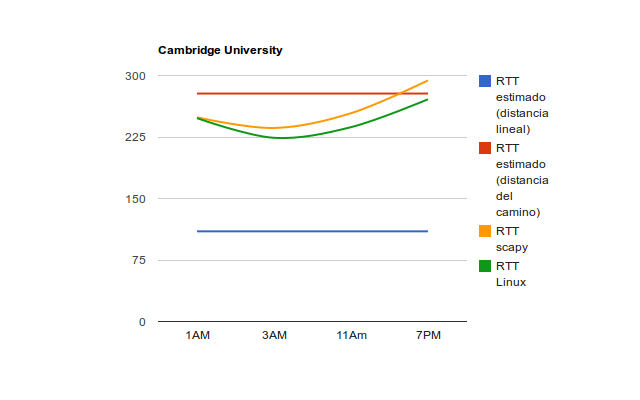
\includegraphics[width=400pt]{cambridge.png}
    \caption{Cambridge University}
    \label{fig:cambridge:count}
\end{figure}

\begin{figure}[h!]
    \centering
    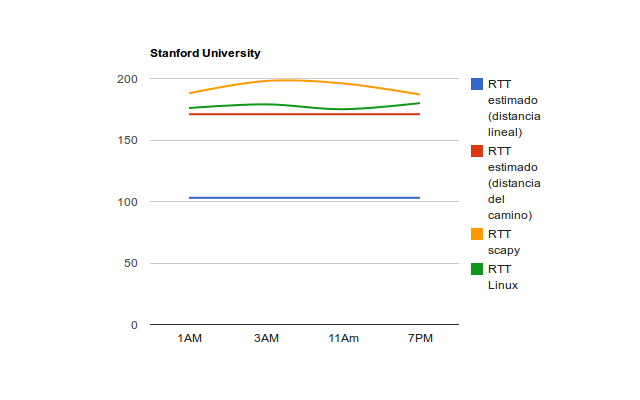
\includegraphics[width=400pt]{stanford.png}
    \caption{Stanford University}
    \label{fig:stanford:count}
\end{figure}

\begin{figure}[h!]
    \centering
    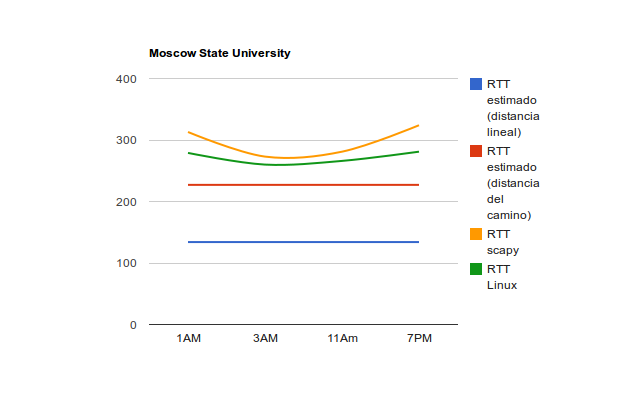
\includegraphics[width=400pt]{msu.png}
    \caption{Moscow State University}
    \label{fig:msu:count}
\end{figure}

\subsection{Análisis de los resultados}
De los gráficos resultantes de los experimentos, pueden observarse varias
cosas que discutiremos a continuación.

En primer lugar, observamos que, efectivamente, el RTT teórico que considera
el camino se acerca más a los valores empíricos que el RTT teórico lineal. La
justificación es, como se dijo antes, que este RTT no asume que el origen y
destino de los experimentos están conectados mediante un medio (fibra óptica)
que los une cubriendo la menor distancia, sino que tiene en cuenta las
desviaciones por los routers intermedios.

No obstante, cabe mencionar que, a diferencia de lo que se esperaba, este RTT
dio, para el caso de la Cambridge University, valores mayores a los empíricos.
Creemos que esto puede deberse a un error en la herramienta de geolocalización
utilizada (hay un desvío de unos 1000 km en uno de los últimos \emph{hops}).
También puede estar sucediendo que ese hop, que tiene una IP de Escocia, en
realidad sea un servidor ubicado en Inglaterra pero que por alguna razón tiene
una IP del primer país. Algo similar ocurre con uno de los primeros hops, que
tiene una IP de Estados Unidos pero el RTT medido a ese host es de 28ms, un
valor más acorde a un host nacional.

Por otro lado, se observa que, en los horarios de la madrugada, hora local, el
RTT disminuye en las dos rutas hacia Europa. Entendemos que esto se debe a que
en esos horarios el tráfico es menor tanto en el origen como en el destino.
Esto no se da de la misma forma en la ruta hacia Estados Unidos, ya que, al
ser en la costa oeste 4 hs menos que en Buenos Aires, a esa hora todavía se
registra un tráfico alto.

Por último, vimos que los resultados de las dos herramientas son bastante
similares. Probablemente el hecho de que la implementación de
\emph{traceroute} del sistema operativo haga 3 intentos por hop sea la razón
por la cual su curva es más suave.

\section{Segunda Parte: Búsqueda de enlaces transatlánticos}
En esta segunda parte, el objetivo es encontrar los enlaces transatlánticos en
las rutas ya estudiadas en la primera parte.

\subsection{Caracterización de los experimentos}
Para esta segunda parte, modificamos nuestra herramienta de \emph{traceroute}
con el objetivo de que esta sea capaz de estimar cuáles de los enlaces pueden
ser transatlánticos. Para esto, se implementó la heurística sugerida que marca
un enlace como transatlántico cuando se cumple que:

$$r > R + m.d$$

siendo:
\begin{itemize}
    \item $r$ la diferencia entre los RTTs de ambas puntas del enlace,
    \item $R$ el promedio de las diferencias de los RTTs entre hops sucesivos
        durante la ejecución del \emph{traceroute},
    \item $d$ el desvío estándar de estas mediciones y
    \item $m$ fijado en 2.
\end{itemize}

\subsection{Resultados de los experimentos}
Lamentablemente en todas los experimentos que realizamos no pudimos identificar ningún enlace transatlántico real pero pudimos distinguir puntos en común entre los experimentos que nos dieron algunos indicios de por qué no los pudimos identificar.\\
Por ejemplo, en la ruta hacia Cambridge notamos un salto muy grande entre dos hops:\\

13 200.89.165.222  BUENOS AIRES, DISTRITO FEDERAL, ARGENTINA   Lat=-34.6132 Long=-58.3772   Time=46.5049743652 ms\\
14 208.178.244.125  BROOMFIELD, COLORADO, UNITED STATES   Lat=39.8828 Long=-105.106   Time=56.2880039215 ms\\
ENLACE TRANSATLANTICO\\
15 67.17.105.238  BROOMFIELD, COLORADO, UNITED STATES   Lat=39.8828 Long=-105.106   Time=161.536931992 ms\\

Claramente no puede haber tanta diferencia entre dos hops tan cerca uno de otro por lo que se nos ocurre que puede ser que haya un host en Argentina con una IP de Estados Unidos y que esté conectado con el siguiente hop mediante un túnel. Lo mismo vimos en las rutas hacia Stanford y Moscú.\\

Otra cosa que nos pareció importante destacar es que en las rutas hacia Cambridge y Moscú siempre apareció un hop que no respondía los mensajes de ping y éste se encontraba antes de un túnel que conectaba Estados Unidos con Europa, ésto es más que una suposición ya que en la ruta obtenida con el traceroute del sistema operativo se ven las etiquetas MPLS:\\
15 po4-40G.ar5.NYC1.gblx.net (67.17.105.238)  182 ms  170 ms po3-40G.ar5.NYC1.gblx.net (67.17.110.254)  206 ms\\
16  * * *\\
17  vlan80.csw3.NewYork1.Level3.net (4.69.155.190) [MPLS: Label 1948 Exp 0]  307 ms\\ vlan70.csw2.NewYork1.Level3.net (4.69.155.126) [MPLS: Label 1947 Exp 0]  270 ms vlan90.csw4.NewYork1.Level3.net (4.69.155.254) [MPLS: Label 1558 Exp 0]  293 ms\\
18  ae-61-61.ebr1.NewYork1.Level3.net (4.69.134.65) [MPLS: Label 1967 Exp 0]  286 ms ae-81-81.ebr1.NewYork1.Level3.net (4.69.134.73)  311 ms *\\
19  ae-41-41.ebr2.London1.Level3.net (4.69.137.65) [MPLS: Label 1638 Exp 0]  352 ms ae-43-43.ebr2.London1.Level3.net (4.69.137.73)  311 ms  558 ms\\
20  vlan101.ebr1.London1.Level3.net (4.69.143.85) [MPLS: Label 1496 Exp 0]  412 ms vlan102.ebr1.London1.Level3.net (4.69.143.89)  336 ms vlan103.ebr1.London1.Level3.net (4.69.143.93)  273 ms\\


\subsection{Conclusiones de los experimentos}
Dados los resultados podemos decir que la heurística propuesta tiene mucho sentido a nivel teórico pero en la práctica no es muy útil para descubrir enlaces transatlánticos.\\
Se nos ocurre que tal vez sería posible buscar los enlaces existentes y tratar de encontrar rutas que pasen por ellos, aún así sería dificil lograr localizar las IPs de los routers de ambas puntas de los enlaces ya que existen túneles que hacen casi imposible saber si se esta usando un enlace u otro.\\


 
\end{document}